\section{Creeping flow through a porous medium}

\begin{figure}[h]
\begin{center}
\framebox{
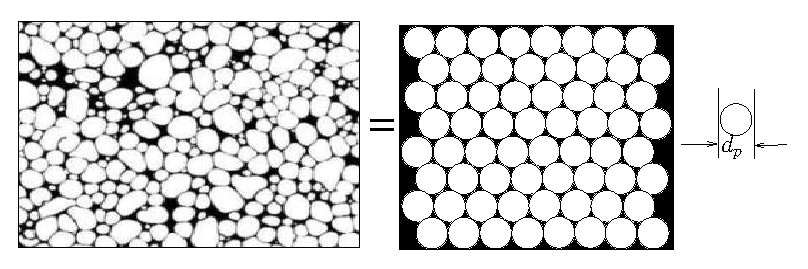
\includegraphics[scale=0.7]{images/c13-porousfig.ps}
}
\end{center}
\caption{Porous medium and its approximation as a bundle of tubes}
\label{pfslfg}
\end{figure}

A porous medium is characterised by the fraction of voids or porosity $\epsilon$. 
$$ \epsilon = \frac{\text{volume of voids}}{\text{volume of porous body}} $$

For a given porosity, the distribution of porosity could be such that the surface area is a second variable. Thus a porous medium is also characterised by surface area per unit volume of solid $S_0$.

$$ S_0 = \frac{\text{wettable surface area}}{\text{volume of solid}} $$

If a porous medium can be imagined to act like a bundle of thin tubes, then the equivalent diameter could be defined as hydraulic radius:

$$ R_h = \frac{\text{volume of voids}}{\text{wettable surface area}}$$

Using the definition of $\epsilon$, volume of voids is $V\epsilon$. Using the definition of $S_0$, the wettable surface area is $S_0 V(1-\epsilon)$.

\begin{equation}
R_h = \frac{\epsilon}{S_0 (1-\epsilon)}
\label{rh}
\end{equation}

If $A$ is the cross sectional area of the porous body, then $A\epsilon$ is the cross sectional area of the voids through which the liquid can flow. If $\bar{u}$ is the actual velocity of the fluid through the void, we can define the average (superficial) velocity $\bar{u}_s$ through the entire porous body such that the volume flow rate $\dot{V}$ is same:

$$ \bar{u}_s A = \bar{u} A\epsilon = \dot{V} $$
or
\begin{equation}
\label{vs}
\bar{u}_s  = \bar{u} \epsilon 
\end{equation}

We take clue from the \textit{Poiseuille flow} the connects the pressure gradient with the flow through a tube:
\begin{equation}
\label{poiseuille}
\bar{u} = \frac{\Delta p}{L} \frac{R^2}{8\mu} = \frac{1}{K_1} \frac{\Delta p}{L} \frac{R^2}{\mu}
\end{equation}

{\bf Darcy's Law}: Considering a porous medium as a bundle of tubes, the volume flow rate is proportional to the cross sectional area and the pressure gradient. The proportionality constant is called as \textit{permeability coefficient}.

\begin{equation}
\label{darcylaw}
\dot{V} = k_D A \frac{\Delta p}{L}
\end{equation}

Considering that the nature of flow through a porous medium is a lot tortuous than through a tube, the constant $K_1$ in equation~\ref{poiseuille} is taken not as $8$ but $4.2$ as has also been validated through experiments.


Now substituting equations \ref{vs}, \ref{rh} into \ref{poiseuille} with $4.2$ as the constant, we get the \textit{Blake-Kozeny equation}:

\begin{equation}
\label{pmflow}
\boxed{
  \bar{u}_s = \frac{1}{4.2} \frac{\Delta p}{L} \frac{\epsilon^3}{\mu S_0^2 \left(1-\epsilon\right)^2}
}
\end{equation}


Validity:

Evaluating $Re$ for porous medium taking the equivalent diameter as $2R_h$,
$$Re = \frac{\bar{u}D\rho}{\mu} = 2 \frac{\rho \bar{u}_s}{\mu S_0 (1-\epsilon)} $$

We define the Reynolds number for porous medium as:

\begin{equation}
\boxed{
   Re_c = \frac{\rho \bar{u}_s}{\mu S_0 (1-\epsilon)}
}
\label{rec}
\end{equation}

The Blake-Kozeny equation is valid for $Re_c < 2$

{\bf Packed bed of spheres}: If the porous medium is made of spherical particles of diameter $d_p$, then $S_0$, the surface area per unit volume of solid can be estimated directly since total wettable area is the sum of surface area of all spheres and total volume of solid is the sum of volume of all spheres.

$$ S_0  = \frac{4 \pi R^2}{\frac{4}{3}\pi R^3} = \frac{3}{R} = \frac{6}{d_p} $$

Substituting this in Blake-Kozeny equation, we get the following equation:

\begin{equation}
\label{ergunp1}
\boxed{
  \frac{\Delta p}{L} = \frac{150 \mu \bar{u}_s \left(1-\epsilon\right)^2}{d_p^2 \epsilon^3}
}
\end{equation}


Evaluating $Re$ for porous medium made of spherical particles (packed bed of spheres) and taking the equivalent diameter as $d_p$,
$$Re = \frac{\bar{u}D\rho}{\mu} = \frac{\rho \bar{u}_s d_p}{\mu 3 (1-\epsilon)} $$

We define the Reynolds number for packed bed of spheres as:

\begin{equation}
\boxed{
   Re_E = \frac{\rho \bar{u}_s d_p}{\mu (1-\epsilon)}
}
\label{rec}
\end{equation}

\section{Exercises}

\begin{enumerate}
 \item Problem 3.12 of~\cite{gp}. Preliminary experimental studies have shown that the porosity in a newly developed packed bed reactor is $\epsilon < 0.6$. The pellets have a diameter of \SI{30}{\milli\metre} and the reducing gas flows through the bed at a rate of \SI{0.025}{\kilo\gram\per\second}. The reactor has \SI{3}{\metre} $\times$ \SI{3}{\metre} square cross section and is \SI{15}{\metre} in height. A constant pressure difference of \SI{690}{\pascal} is maintained between the inlet and outlet nozzles, and it may be assumed that the temperature is uniform throughout the reactor. You are required to evaluate the bed porosity. The properties of the gas are $\mu$ = \SI{2.07e-5}{\pascal\second} and $\rho$ = \SI{1.2}{\kilo\gram\per\metre\cubed}. Comment if the solution is valid. \\
{\it Answer}: $\epsilon = 0.054$.

\end{enumerate}



%%%%%%%%%%%%%%%%%%%%%%%%%%%%%%%%%%%%%%%%%%%%%%%%%%%%%%%%%%%%%%%%%%%%%%%%%%

